\section{Power}
\label{sec:power}
\textit{\hyperlink{schematic.8}{schematic}}

\fixme{I think this section needs information about PSRRs, especially for regulators that feed RF
  circuits.}

\fixme{Another thing that needs clarification is where should the LDO's be placed? Should they be
  located near the loads they serve or the switching converters? My guess would be near the
  converters since that decreases the part of the board that is exposed to the switching noise.}

\subsection{Overview}
\label{sec:power-overview}

A barrel jack is used to feed a 12V input to the board which is then administered to a 10V output
linear regulator and two buck converters that output 5.6V and 3.6V. The buck converters in turn pass
their voltages on to several LDO voltage regulators for input to the various digital ICs on the
board. The benefit of chaining switching converters to linear regulators is greater energy
efficiency and better noise suppression than can be achieved by using either alone. An LED indicates
when power is administered to the board.

\subsection{Barrel Jack / Power Input}
\label{sec:power-input}

A ferrite bead pi filter is placed at the output of the barrel jack connection. The ferrite bead is
rated for $5.1A$, which is more than double the absolute max current draw of the radar. The barrel
connector is a switched jack, but we do not use a battery on this PCB so the 3rd pin is grounded.

\subsection{TPS5420D Buck Converter}
\label{sec:tps5420d}

\subsubsection{Description}
\label{sec:tps5420d-description}

The TPS5420D is an internally-compensated buck converter with a fixed switching frequency of
$500\si{kHz}$, whose block diagram is shown in Figure~\ref{fig:tps5420d-block}. The converter first
compares the divided voltage output with a $1.221V$ reference and uses an error amplifier to amplify
the difference. It then feeds that difference into a PWM comparator along with a sawtooth ramp
waveform. If the PWM comparator outputs a high voltage the switch is turned off, effectively
decreasing the duty cycle. Conversely, a low voltage saturates the transistor and increases the duty
cycle. This has the effect of converging the output voltage to its set point. The TPS5420 has a ramp
time of between $6.6$ and $10 \si{ms}$.

\begin{figure}[h]
        \centering
        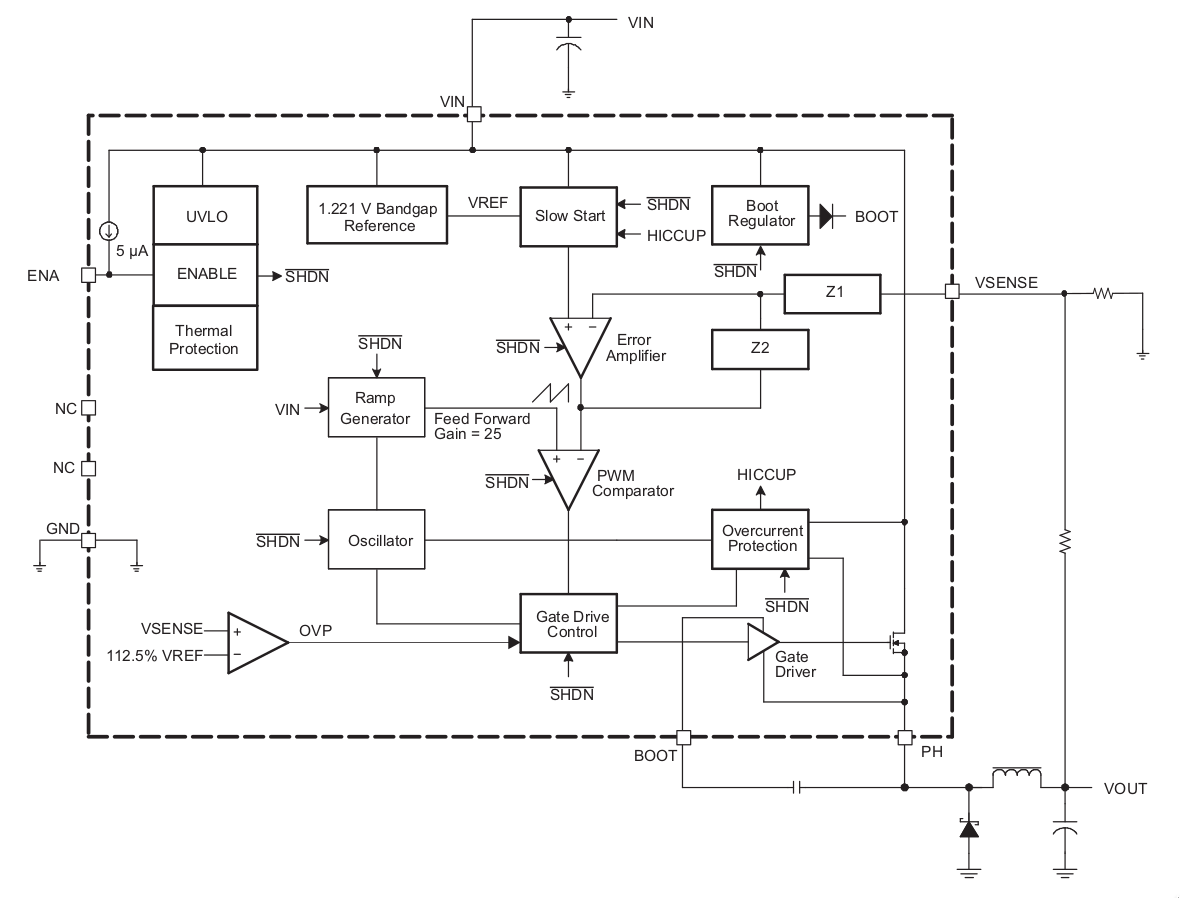
\includegraphics[width=0.9\textwidth]{data/tps5420d-block-diagram}
        \caption{TPS5420D Block Diagram}
        \label{fig:tps5420d-block}
\end{figure}

\subsubsection{Pinout}
\label{sec:tps5420d-pinout}

\fixme{What is the point of BOOT?}
\label{tab:tps5420d-pinout}
\begin{tabularx}{\textwidth}{l l X}
        \caption{TPS5420D pinout.}                                                               \\
        \toprule
        \textbf{\#} & \textbf{Pin} & \textbf{Description}                                        \\
        \midrule
        1           & BOOT         &                                                             \\
        2, 3        & NC           & No connect.                                                 \\
        4           & VSENSE       & Feedback voltage for the regulator. This compares the divided output with a 1.221V
        reference.                                                                               \\
        5           & ENA          & Enable pin. This can be left floating to enable the device. \\
        6           & GND          & Ground.                                                     \\
        7           & VIN          & Input supply voltage.                                       \\
        8           & PH           & Output voltage.                                             \\
        \bottomrule
\end{tabularx}

\subsubsection{Component Selection}
\label{sec:tps5420d-component-selection}

An inductor is chosen such that it satisfies the following 3 requirements:
\begin{enumerate}
\item The inductance is given by Equation~\ref{eq:buck-inductance}.
\item The current rating is at least 2x the maximum load current.
\item The self-resonant frequency is at least 10x the switching frequency.
\end{enumerate}

\begin{equation}
        \label{eq:buck-inductance}
        L_{\text{min}} = \frac{T}{2} \frac{V_{\text{out}}}{I_{\text{out(min)}}} \left(1 -
                \frac{V_{\text{out}}}{V_{\text{in}}}\right)
\end{equation}

The requirements are given in Table~\ref{tab:buck-inductor-reqs}. All of these requirements are
satisfied by the \href{https://www.bourns.com/docs/Product-Datasheets/SRR1210A.pdf}{SRR1210A-330M}
$33\si{\mu H}$ Bourns ferrite bead.

\label{tab:buck-inductor-reqs}
\begin{tabularx}{\textwidth}{c c c c}
        \caption{TPS5420D inductor requirements. I've assumed an input ripple of $300\si{mV}$.} \\
        \toprule
        \textbf{Buck Vout} & \textbf{Lmin}    & \textbf{Current Rating} & \textbf{SRF min}      \\
        \midrule
        \endhead
        $5.6\si{V}$        & $6.5\si{\mu H}$  & $2.21\si{A}$            & $5\si{MHz}$           \\
        $3.6\si{V}$        & $15.1\si{\mu H}$ & $2.50\si{A}$            & $5\si{MHz}$           \\
        \bottomrule
\end{tabularx}

The input, output and boot capacitors were chosen by the \href{https://webench.ti.com}{WEBENCH
  tool}. The flyback diode was chosen to support $2A$ of current.

\subsubsection{Downstream Current Draw}
\label{sec:tps5420d-current}

It is important to know both the maximum and minimum current draw of components whose voltage inputs
are fed by the output of a buck converter. The minimum current sets a lower bound on the inductance
that can be used (see Equation~\ref{eq:buck-inductance}) since the converter must remain in CCM for
proper operation. It is also important to ensure that the buck converter and inductor are rated for
the maximum current draw of downstream devices. Saturating the ferrite-core inductor can cause a
loss in inductance.

\label{tab:buck-5.6-current}
\begin{tabularx}{\textwidth}{l c c X>{\raggedright\arraybackslash}X}
        \caption{The current draw of components downstream from the 5.6V buck converter. When
          minimum current draw is omitted from the datasheet I've assumed 0A.}                                                 \\
        \toprule
        \textbf{MFN}                     & \textbf{I\textsubscript{Q}} & \textbf{I\textsubscript{max}} &
        \textbf{Voltage Inputs}                                                                                                \\
        \midrule
        \hyperlink{sec:adl5802}{ADL5802} & $170\si{mA}$                & $300\si{mA}$                  & 5V                    \\
        \hyperlink{sec:adf4158}{ADF4158} & $312.5\si{\mu A}$           & $5\si{mA}$                    & 5V (VP)               \\
        \hyperlink{sec:se5004l}{SE5004L} & $300\si{mA}$                & $800\si{mA}$                  & 5V (VCC1, VCC2, VCC3) \\
        \midrule
        Total                            & $470\si{mA}$                & $1.105\si{A}$                 & -                     \\
        \bottomrule
\end{tabularx}

\label{tab:buck-3.6-current}
\begin{tabularx}{\textwidth}{l c c X>{\raggedright\arraybackslash}X}
        \caption{Components downstream from the 3.6V buck converter.} \\
        \toprule
        \textbf{MFN} & \textbf{I\textsubscript{Q}} & \textbf{I\textsubscript{max}} & \textbf{Voltage
          Inputs} \\
        \midrule
        \hyperlink{sec:kt2520k}{KT2520K}  & - & $2\si{mA}$ & 1.8V \\
        \hyperlink{sec:nc7s04}{NC7S04} & $1\si{\mu A}$ & $12.5\si{mA}$ & 3.3V \\
        \hyperlink{sec:nb3n551}{NB3N551} & - & $40\si{mA}$ & 3.3V \\
        \midrule
        \hyperlink{sec:xc7a15t-ftg256}{XC7A15T-FTG256} & $97\si{mA}$ & $277\si{mA}$ & 1V (VCCINT,
        VCCBRAM) \\
        XC7A15T-FTG256 & $22\si{mA}$ & $87\si{mA}$ & 1.8V (VCCADC, VCCAUX) \\
        XC7A15T-FTG256 & $1\si{mA}$ & $201\si{mA}$ & 3.3V (VCC0) \\
        \hyperlink{sec:w25q32jv}{W25Q32JV} & $10\si{\mu A}$ & $25\si{mA}$ & 3.3V \\
        \midrule
        \hyperlink{sec:ft2232h}{FT2232H} & $510\si{\mu A}$ & $280\si{mA}$ & 3.3V (VPHY, VPLL, VCORE,
        VCCIO) \\
        \hyperlink{sec:93lc46b}{93LC46B} & - & $2\si{mA}$ & 3.3V \\
        \midrule
        \hyperlink{sec:ltc2292}{LTC2292} & $5\si{mA}$ & $95\si{mA}$ & 3.3V (OVDD), 3V (VDD) \\
        \midrule
        \hyperlink{sec:ada4940-2}{ADA4940-2} & $4.2\si{mA}$ & $5.52\si{mA}$ & 3.3V \\
        \midrule
        \hyperlink{sec:adf4158}{ADF4158} & - & $32\si{mA}$ & 3.3V (AVDD, DVDD) \\
        \midrule
        \hyperlink{sec:hmc431lp4}{HMC431LP4} & $19\si{mA}$ & $27\si{mA}$ & 3V \\
        \midrule
        \hyperlink{sec:trf37a73}{TRF37A73} & $250\si{\mu A}$ & $130\si{mA}$ & 3V \\
        \hyperlink{sec:sky65404}{SKY65404} & $20\si{mA}$ & $36\si{mA}$ & 3V (VENABLE, VCC) \\
        \midrule
        Total & $169\si{mA}$ & $1.252\si{A}$ & - \\
        \bottomrule
\end{tabularx}

\subsubsection{PCB Layout}
\label{sec:tps5420d-pcb}

The datasheet provides a suggested PCB layout, shown in Figure~\ref{fig:tps5420d-pcb}.

\begin{figure}[h]
        \centering
        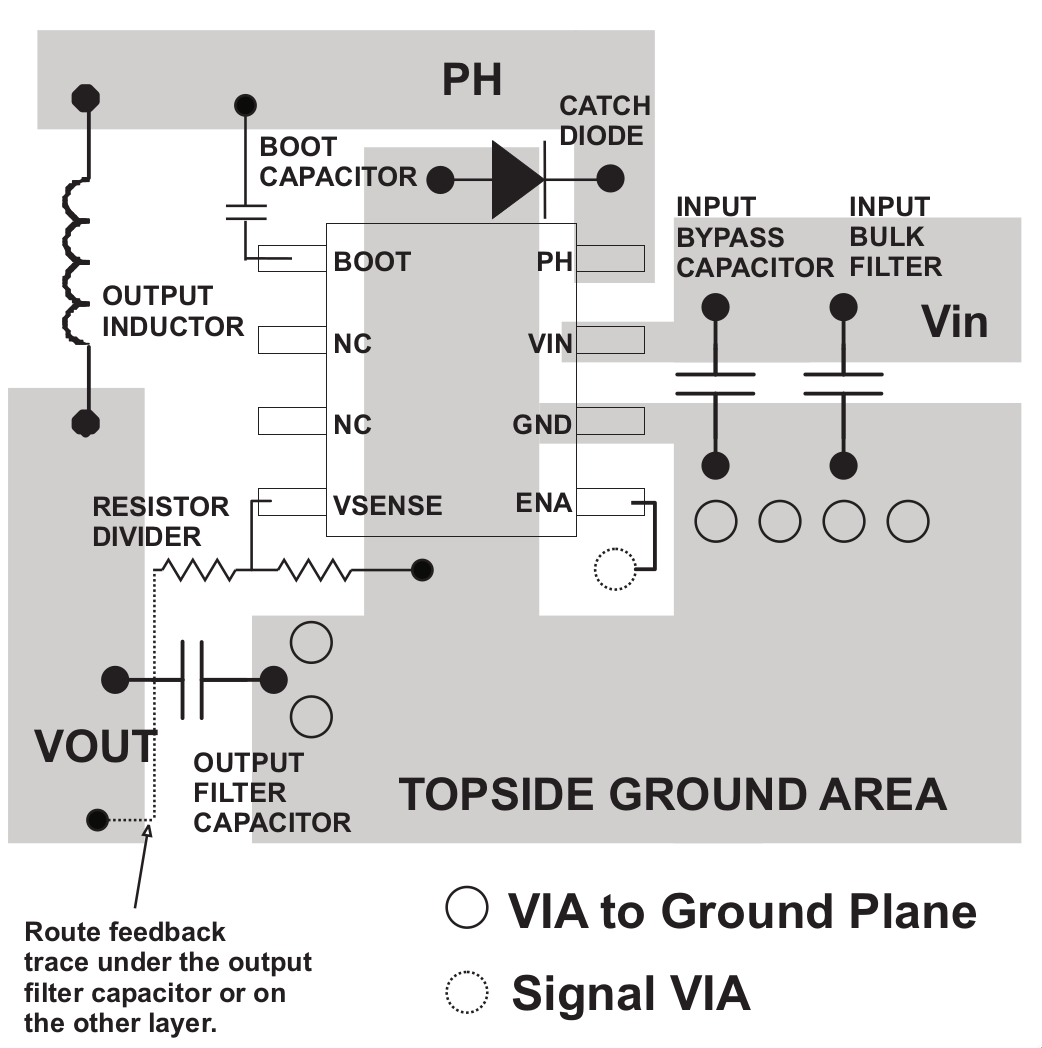
\includegraphics[width=0.75\textwidth]{data/tps5420d-pcb.png}
        \caption{TPS5420D suggested PCB layout.}
        \label{fig:tps5420d-pcb}
\end{figure}

\subsection{TPS560200 Buck Converter}
\label{sec:tps560200}

\subsubsection{Description}
\label{sec:tps560200-description}

The TPS560200 is an internally-compensated buck converter with a switching frequency of
$600 \si{kHz}$ and a fixed ramp time of $2 \si{ms}$. It is needed, rather then a linear regulator
chained to a TPS5420D, because the FPGA requires its $1 \si{V}$ power supply first.

\subsubsection{Pinout}
\label{sec:tps560200-pinout}

\label{tab:tps560200-pinout}
\begin{tabularx}{\textwidth}{l l X}
        \caption{TPS50600 pinout.}                                                 \\
        \toprule
        \# & Pin    & Description                                                  \\
        \midrule
        1  & EN     & Enable pin. Can be floated to unconditionally enable device. \\
        2  & GND    & Ground.                                                      \\
        3  & PH     & Output voltage.                                              \\
        4  & VIN    & Input voltage.                                               \\
        5  & VSENSE & Feedback, compared to a $0.8 \si{V}$ reference.              \\
        \bottomrule
\end{tabularx}

\subsubsection{Component Selection}
\label{sec:tps560200-component-selection}

The voltage divider resistors, filter capacitors and input capacitors are specified by the
datasheet. The output voltage ripple must be sufficiently small that it falls within the required
voltage range of the FPGA's V\textsubscript{CCINT} input. Specifically, it must be less than
$100 \si{mV}$. Texas Instruments provides\footnote{\url{www.ti.com/lit/an/slva630a/slva630a.pdf}} an
equation for the voltage ripple of a buck converter, given a small capacitor resistance. I'm further
assuming an ESR of 0 since I'm using ceramic capacitors at the output and the current draw is fairly
low. The equation is provided in Equation~\ref{eq:tps560200-ripple-voltage}. The ripple current for
a buck converter is given in Equation~\ref{eq:tps560200-ripple-current}. Finally, the remaining
inductor requirements are specified in Table~\ref{tab:tps560200-inductor-reqs}. All of these
requirements are satisfied by a $10 \si{\mu H}$ inductor, which is used in the datasheet. However,
this puts the inductor a bit close to DCM and since I have extra $33 \si{\mu H}$ inductors on hand
I'd rather be safe and use one of those.

\begin{equation}
        \label{eq:tps560200-ripple-voltage}
        V_{\text{p2p}} = \frac{I_{\text{p2p}}}{8 C F_{\text{SW}}}
\end{equation}

\begin{equation}
        \label{eq:tps560200-ripple-current}
        I_{\text{p2p}} = V_{\text{out}} \frac{1 - D}{L F_{\text{SW}}}
\end{equation}

\label{tab:tps560200-inductor-reqs}
\begin{tabularx}{\textwidth}{c c c c}
        \caption{TPS560200 inductor requirements.}                                            \\
        \toprule
        V\textsubscript{out} & L\textsubscript{min} & Current Rating & SRF\textsubscript{min} \\
        \midrule
        $1 \si{V}$           & $7.9 \si{\mu H}$     & $554 \si{mA}$  & $6 \si{MHz}$           \\
        \bottomrule
\end{tabularx}

\subsubsection{Downstream Current Draw}
\label{sec:tps560200-current}

\label{tab:tps560200-current}
\begin{tabularx}{\textwidth}{l c c X}
        \caption{Components downstream from the TPS560200 buck converter.} \\
        \toprule
        MFN & I\textsubscript{Q} & I\textsubscript{max} & Voltage Inputs \\
        \midrule
        \hyperlink{sec:xc7a15t-ftg256}{XC7A15T-FTG256} & $97\si{mA}$ & $277\si{mA}$ & 1V (VCCINT,
        VCCBRAM) \\
        \bottomrule
\end{tabularx}

\subsubsection{PCB Layout Guidelines}
\label{sec:tps560200-pcb}

The datasheet provides a recommended layout, shown in Figure~\ref{fig:tps560200-pcb}.

\begin{figure}[h]
        \centering
        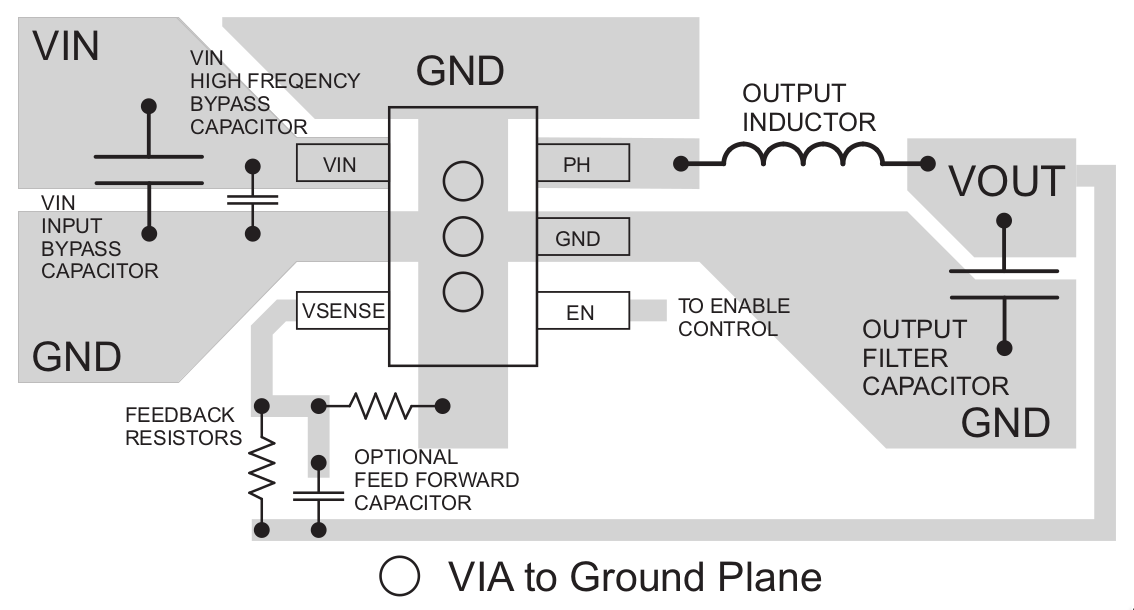
\includegraphics[width=0.75\textwidth]{data/tps560200-pcb}
        \caption{TPS560200 recommended PCB layout.}
        \label{fig:tps560200-pcb}
\end{figure}

\subsection{LP2985A-10DBVR Linear Regulator}
\label{sec:lp2985a-10dbvr}

\subsubsection{Description}
\label{sec:lp2985a-10dbvr-description}

The LP2985A is a low-dropout fixed-output regulator with a max output current of $150\si{mA}$. It's
functional block diagram is shown in Figure~\ref{fig:lp2985a-block-diagram}. It uses an op-amp to
compare the voltage-divided output with a $1.23\si{V}$ reference. It then turns a PNP transistor
on/off depending on the output voltage level relative to its $10\si{V}$ target.

\begin{figure}[h]
        \centering
        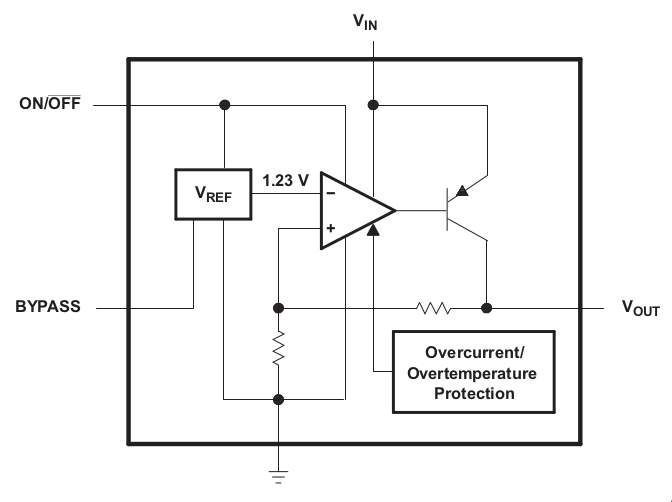
\includegraphics[width=0.5\textwidth]{data/lp2985a-block-diagram}
        \caption{The LP2985A-10DBVR LDO regulator block diagram.}
        \label{fig:lp2985a-block-diagram}
\end{figure}

\subsubsection{Pinout}
\label{sec:lp2985a-10dbvr-pinout}

\label{tab:lp2985a-10dbvr-pinout}
\begin{tabularx}{\textwidth}{l l X}
        \caption{LP2985A's pin descriptions.}							\\
        \toprule
        \textbf{\#}	&	\textbf{Pin}		&	\textbf{Description}		\\
        \midrule
        1		&	VIN			&	Voltage supply.			\\
        2		&	GND			&	Ground.				\\
        3		&	ON/\textoverline{OFF}	&	Active-low shutdown pin. It is tied
	to VIN since the device should be unconditionally enabled. \\
        4		&	BYPASS			&	Connected to a $10\si{nF}$ capacitor
	to ground to decrease output voltage noise. \\
        5		&	VOUT			&	Regulated, voltage output.	\\
        \bottomrule
\end{tabularx}

\subsubsection{Component Selection}
\label{sec:lp2985a-10dbvr-component-selection}

The input capacitor should be at least $1\si{\mu F}$ and the output capacitor should be at least
$2.2\si{\mu F}$, but higher values are better at the output. I'm using $10\si{\mu F}$.

\subsubsection{Downstream Current Draw}
\label{sec:lp2985a-10dbvr-current}

\label{tab:lp2985a-10dbvr-current}
\begin{tabularx}{\textwidth}{l c c X}
        \caption{Downstream current draw for the 10V linear regulator.} \\
        \toprule
        MFN & I\textsubscript{Q} & I\textsubscript{max} & Voltage Inputs \\
        \midrule
        \hyperlink{sec:tlv172dck}{TLV172DCK} & $1.6\si{mA}$ & $75\si{mA}$ & 10V \\
        \bottomrule
\end{tabularx}

\subsubsection{PCB Layout}
\label{sec:lp2985a-10dbvr-pcb}

The input and output capacitors should be placed within $1\si{cm}$ of the input and output pins and
have a low-impedance path to ground.

\subsection{TPS7A91 LDO Voltage Regulator}
\label{sec:tps7a91}

\subsubsection{Description}
\label{sec:tps7a91-description}

The TPS7A91 is a low-noise, low-dropout and adjustable voltage regulator. It has an RMS output noise
of $4.7 \si{\mu V}$. The regulator works by comparing the feedback voltage, at the inverting input
of an error amplifier, with a $0.8 \si{V}$ reference voltage at the non-inverting input. The output
of the error amplifier is connected to the gate of an n-channel MOSFET whose drain is attached to
the input voltage and whose source is attached to the output voltage. This negative feedback creates
a stable equilibrium when the output voltage is at its set-point. The functional block diagram is
shown in Figure~\ref{fig:tps7a91-block-diagram}.

The power-good function of one regulator is used to ensure that the $1.8 \si{V}$ supply arrives at
the FPGA before the $3.3 \si{V}$ supply. The circuit uses an open-drain output with a pull-up
resistor. If the output voltage goes below some threshold, the MOSFET will saturate and the PG line
will be brought low. Otherwise, it will be pulled high.

\begin{figure}[h]
        \centering
        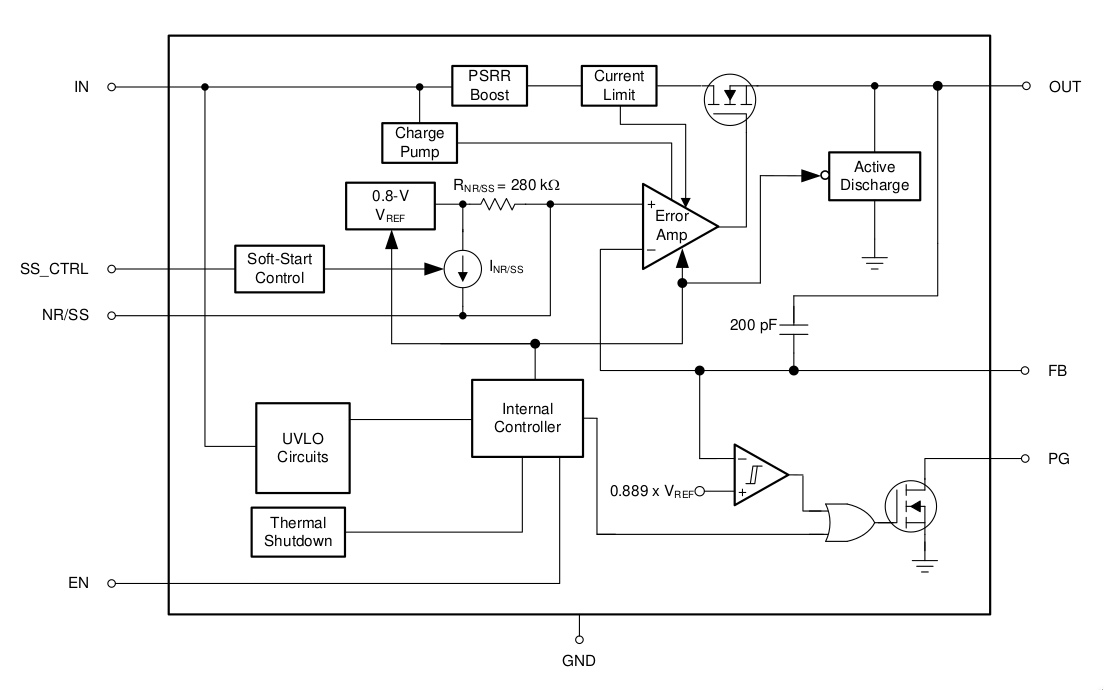
\includegraphics[width=0.75\textwidth]{data/tps7a91-block-diagram}
        \caption{TP7A91 block diagram.}
        \label{fig:tps7a91-block-diagram}
\end{figure}

\subsubsection{Pinout}
\label{sec:tps7a91-pinout}

\label{sec:tps7a91-pinout}
\begin{tabularx}{\textwidth}{l l X}
        \caption{TPS7A91 pinout.} \\
        \toprule
        \# & Pin & Description \\
        \midrule
        1, 2 & OUT & Regulated output voltage. A $10 \si{\mu F}$ or greater
        capacitor should be
        connected between this pin and ground. \\
        3 & FB & Feedback pin. The divided output voltage is compared against a $0.8 \si{V}$
        reference. \\
        4 & GND & Ground. \\
        5 & PG & A power good indicator that can signal to downstream devices when voltage is within
        some range of the desired level. The design doesn't use this and so the pin has been left
        floating. \\
        6 & SS\_CTRL & Soft-start control pin. Tying this pin to the input voltage increases the
        soft-start charging current to $100 \si{\mu A}$, which reduces the startup time. This pin
        could have also been tied to ground if a slower startup time was desired. \\
        7 & EN & Enable. Tying this to the input voltage unconditionally enables this device. \\
        8 & NR/SS & Noise-reduction pin. A capacitor can be placed between this pin and ground
        to reduce output noise. This effectively acts like an RC filter. A capacitance between $10
        \si{nF}$ and $1 \si{\mu F}$ is recommended. I've used $100 \si{nF}$. This pin also limits
        inrush current. \\
        9, 10 & IN & Input voltage pin. A bypass capacitor of $10 \si{\mu F}$ or more is
        required. \\
        \bottomrule
\end{tabularx}

\subsubsection{Component Selection}
\label{sec:tps7a91-component-selection}

MLCC capacitors are recommended for input and output bypassing due to their low ESR, with
preferences given to X5R and X7R types. Additionally, they should be derated by at least 50\%. The
recommended capacitance is $10 \si{\mu F}$ or greater at the input and output. I've used
$10 \si{\mu F}$ at the input and the same at the output, with the option for another capacitor at
the output if needed. The $10 \si{nF}$ feed-forward capacitor between FB and OUT is recommended by
the datasheet to improve noise and PSRR performance. The voltage divider resistors are specifically
mentioned in the datasheet to get the appropriate output values.

\subsubsection{PCB Layout}
\label{sec:tps7a91-pcb}

The recommended PCB layout is shown in Figure~\ref{fig:tps7a91-pcb}.

\begin{figure}[h]
        \centering
        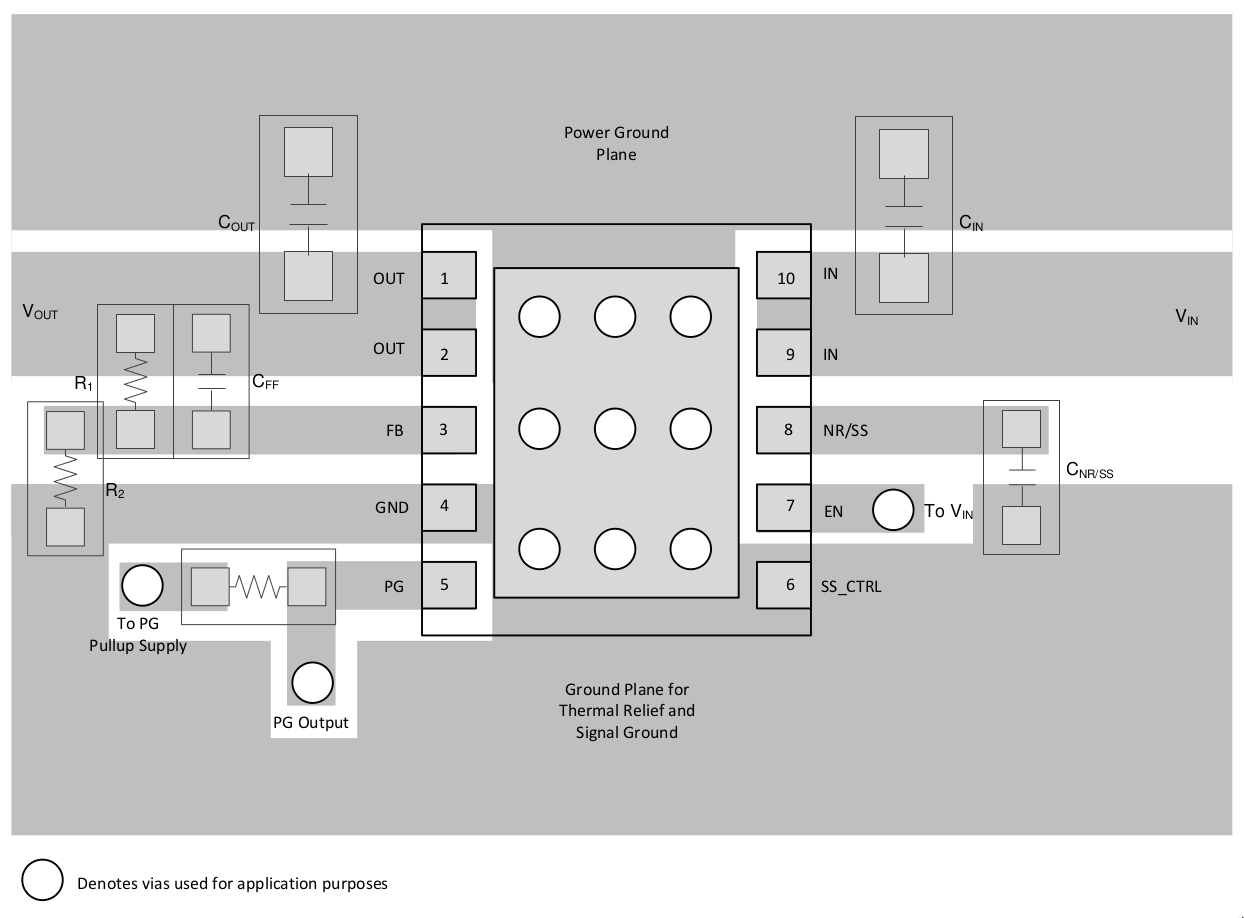
\includegraphics[width=0.75\textwidth]{data/tps7a91-pcb}
        \caption{TPS7A91 recommended PCB layout.}
        \label{fig:tps7a91-pcb}
\end{figure}

\subsection{TPS7A7001DDA LDO Regulator}
\label{sec:tps7a7001dda}

\subsubsection{Description}
\label{sec:tps7a7001dda-description}

The TPS7A7001DDA supports low dropouts up to $2 \si{A}$, which is important since it must
accommodate a maximum current draw of $1.1 \si{A}$ (see Table~\ref{tab:buck-5.6-current}).

\subsubsection{Pinout}
\label{sec:tps7a7001dda-pinout}

\label{tab:tps7a7001dda-pinout}
\begin{tabularx}{\textwidth}{l l X}
        \caption{TPS7A7001DDA pinout.}                                \\
        \toprule
        \#      & Pin & Description                                   \\
        \midrule
        1, 4, 5 & NC  & No connect.                                   \\
        2       & EN  & Enable input. Connected to IN since unused.   \\
        3       & IN  & Input voltage.                                \\
        6       & OUT & Regulated voltage output.                     \\
        7       & FB  & Feedback, compared to $0.5 \si{V}$ reference. \\
        8       & GND & Ground.                                       \\
        9       & EP  & Exposed pad. Tied to ground.                  \\
        \bottomrule
\end{tabularx}

\subsubsection{Component Selection}
\label{sec:tps7a7001dda-component-selection}

An input capacitor of $1 - 10 \si{\mu F}$ and with low ESR is recommended. The output capacitor
should be ceramic and can be anywhere from $4.7 - 47 \si{\mu F}$. I've chosen $10 \si{\mu F}$ with
the option for an additional capacitor if needed. The voltage divider resistors are specifically
recommended by the datasheet.

\subsubsection{PCB Layout}
\label{sec:tps7a7001dda-pcb}

The recommended PCB layout is provided in~\ref{fig:tps7a7001dda-pcb}.

\begin{figure}[h]
        \centering
        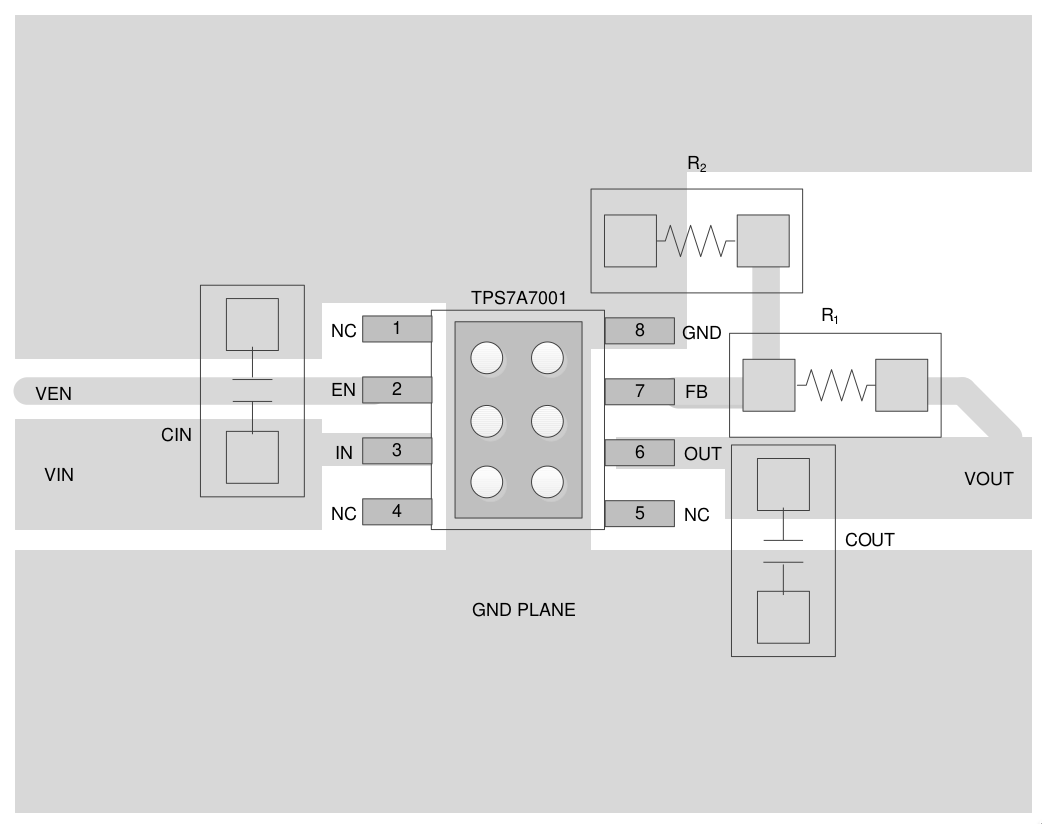
\includegraphics[width=0.75\textwidth]{data/tps7a7001dda-pcb}
        \caption{TPS7A7001DDA recommended PCB layout.}
        \label{fig:tps7a7001dda-pcb}
\end{figure}

\subsection{LP5907MFX-3.0}
\label{sec:mic5301-3.3}

\subsubsection{Description}
\label{sec:mic5301-3.3-description}

The LP5907MFX-3.0 is a low-noise and dropout voltage regulator used to power the VCO and
reception-side amplifiers. It has a current rating of $250 \si{mA}$ which is more than the maximum
current load of the downstream components.

\subsubsection{Pinout}
\label{sec:lp5907mfx-3.0-pinout}

\label{tab:lp5907mfx-3.0-pinout}
\begin{tabularx}{\textwidth}{l l X}
        \caption{LP5907MFX-3.0 pinout.}                                      \\
        \toprule
        \# & Pin & Description                                               \\
        \midrule
	1  & IN  & Voltage input.                                            \\
	2  & GND & Ground.                                                   \\
	3  & EN  & Enable. Tied to IN to keep the device unconditionally on. \\
	4  & NC  & No connect.                                               \\
	5  & OUT & $1.8 \si{V}$ output.                                      \\
        \bottomrule
\end{tabularx}

\subsubsection{Component Selection}
\label{sec:lp5907mfx-3.0-component-selection}

The input and output capacitors should be $1 - 10 \si{\mu F}$, with the input capacitor at least as
large as the output capacitor. I've used $10 \si{\mu F}$ capacitors in this design.

\subsubsection{PCB Layout}
\label{sec:lp5907-3.0-pcb}

The recommended PCB layout is shown in Figure~\ref{fig:lp5907mfx-3.0-pcb}.

\begin{figure}[h]
	\centering
	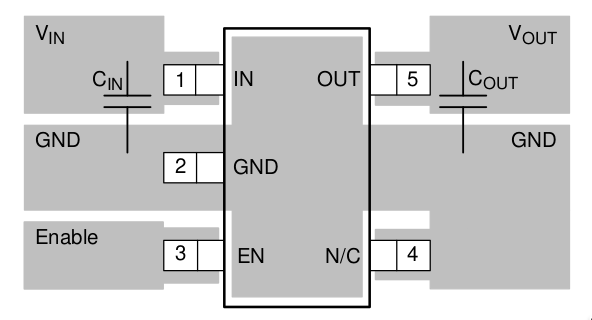
\includegraphics[width=0.5\textwidth]{data/lp5907mfx-3-pcb}
	\caption{LP5907MFX-3.0 recommended PCB layout.}
	\label{fig:lp5907mfx-3.0-pcb}
\end{figure}

%%% Local Variables:
%%% mode: latex
%%% TeX-master: "fmcw-radar"
%%% End:
